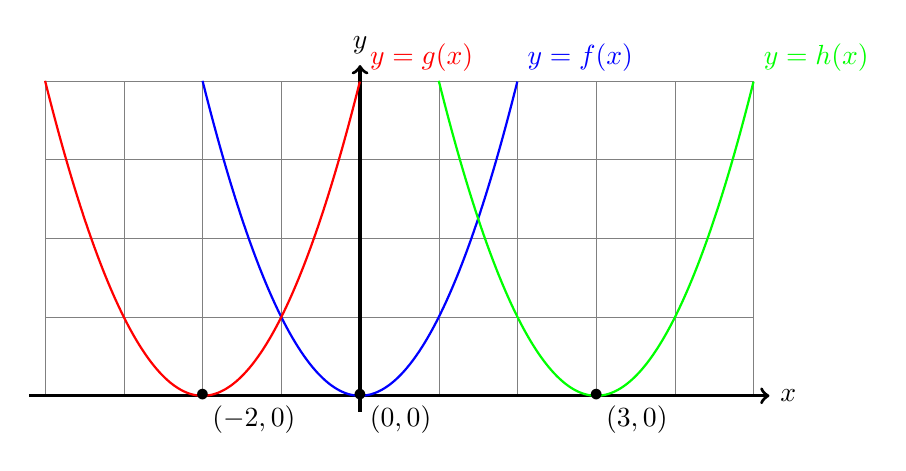
\begin{tikzpicture}
  \draw[very thin,color=gray] (-4,0) grid (5,4);

  \draw[very thick,->] (-4.2,0) -- (5.2,0) node[right] {$x$};
  \draw[very thick,->] (0,-.2) -- (0,4.2) node[above] {$y$};
  
  \draw [color=blue,thick] plot[smooth,samples=500,domain=-2:2] (\x,{(\x)^2}) node [above right] {$y = f(x)$};
  \draw [color=red,thick] plot[smooth,samples=500,domain=-4:0] (\x,{(\x+2)^2}) node [above right] {$y = g(x)$};
  \draw [color=green,thick] plot[smooth,samples=500,domain=1:5] (\x,{(\x-3)^2}) node [above right] {$y = h(x)$};

  \node at (0,0) {$\bullet$};
  \node [below right] at (0,0) {$(0,0)$};

  \node at (-2,0) {$\bullet$};
  \node [below right] at (-2,0) {$(-2,0)$};

  \node at (3,0) {$\bullet$};
  \node [below right] at (3,0) {$(3,0)$};
\end{tikzpicture}
